
\documentclass[12pt]{article}
\usepackage[paper=letterpaper, margin=0.8in]{geometry}

%% The graphicx package provides the includegraphics command.
\usepackage{graphicx}
%% The amssymb package provides various useful mathematical symbols
\usepackage{amssymb}
%% fix strange gensymb error
\usepackage{textcomp}
%% symbols, especially degree
\usepackage{gensymb}
%% scientific units
\usepackage{siunitx}
%% line spacing
\usepackage{setspace}
\doublespacing
%% put figures at the end
%\usepackage[nomarkers]{endfloat}
%% allow hyperlinks
\usepackage{hyperref}
%% color comments
\usepackage{soul}
\usepackage{color}
%% left justification in tables
\usepackage{array}
\newcolumntype{P}[1]{>{\raggedright\arraybackslash}p{#1}}
%%references
\usepackage{natbib}
\setcitestyle{numbers}
\usepackage{pdflscape}

%stop hbox nonesense
\tolerance=1600

\usepackage{lineno}

\begin{document}

%stop indents
\setlength\parindent{0pt}% globally suppress indentation

{\Large
\textbf\newline{Carry-over effects of larval microclimate on the transmission potential of a mosquito-borne pathogen}}

\bigskip

Michelle V. Evans\textsuperscript{1,2,3*},
Justine C. Shiau\textsuperscript{4},
Nicole Solano\textsuperscript{1,2},
Melinda A. Brindley\textsuperscript{4,5},
John M. Drake\textsuperscript{1,2},
Courtney C. Murdock\textsuperscript{1,2,3,4,6,7}
\smallskip


\textbf{1} Odum School of Ecology, University of Georgia, Athens, GA, USA
\newline
\textbf{2} Center for the Ecology of Infectious Diseases, University of Georgia, Athens, GA, USA
\newline
\textbf{3} Center for Tropical Emerging Global Diseases, University of Georgia, Athens, GA, USA
\newline
\textbf{4} Department of Infectious Disease, University of Georgia, Athens, GA, USA
\newline
\textbf{5} Department of Population Health, University of Georgia, Athens, GA, USA
\newline
\textbf{6} Center for Vaccines and Immunology, University of Georgia, Athens, GA, USA
\newline
\textbf{7} River Basin Center, University of Georgia, Athens, GA, USA
\smallskip

\noindent
*Corresponding Author: mvevans@uga.edu
\bigskip

\newpage

\textbf{Abstract} Climate shapes the transmission of mosquito-borne pathogens through impacts on both the vector and the pathogen.  In addition to direct effects of the present environment, indirect carry-over effects from previous life history stages can influence mosquito life history traits relevant to disease transmission. While this has been explored in a laboratory setting, the net effect of temperature-mediated carry-over effects due to relevant environmental variation in the larval stage is ambiguous. Here, we use data collected from a semi-field experiment investigating dengue dynamics in \textit{Aedes albopictus} across a relevant environmental gradient to parameterize a dengue transmission model. We reared \textit{Ae. albopictus} across three different land classes characterized by their proportion of impervious surface. Emerged females were offered a dengue infectious bloodmeal, kept at a constant 27C, and assayed for infection, dissemination, and infectiousness 21 days post infection. Incorporating carry-over effects of larval environment on measures of vector competence resulted in lower predicted dengue transmission potential across land class and season, however a strong positive relationship with larval environmental temperature remained. Given the significant impact of carry-over effects on predicted transmission potential, we suggest that future mechanistic models of disease transmission include both direct and carry-over effects of environmental temperature.

\smallskip

\textbf{Keywords:} carry-over effects, dengue, mosquito ecology, urban microclimate

\linenumbers
\doublespacing
%add indents back in
\setlength\parindent{20pt}%

\newpage

\section{Introduction}

Climate plays an important role in the transmission of mosquito-borne pathogens, determining the geographic range of disease vectors and shaping transmission dynamics. Variation in environmental conditions can drive indivudal-level variation in character traits relevant to mosquito popuation dynamics \citep{delatte2009, yang2009, alto2001}, as well as pathogen transmission \citep{murdock2012}. However, in addition to the direct effects of the current environment, mosquito phenotype (including fitness) is shaped indirectly by the environmental conditions experienced in previous life history stages, a phenomenon known as carry-over effects \citep{harrison2011}. Carry-over effects have been documented in a wide-range of species with complex life cycles, such as amphibians \citep{vonesh2005}, migratory birds \citep{norris2006}, and insects \citep{deblock2005a}. Similarly, the mosquito life cycle is characterized by ontogenetic niche shifts, with a larval aquatic stage and an adult terrestrial stage. Following these studies, we reason that the thermal environment a mosquito experiences during its larval stage is likely to have lasting impacts on its adult traits, and, ultimately, on transmission potential.

There are several pathways by which carry-over effects from the larval environment might impact key adult traits that are relevant for overall fitness and disease transmission. If the larval environment is of low quality (e.g. resource scarcity or thermal stress, or crowding), individuals may experience developmental constraints that negatively impact adult fitness \citep{inger2010}. For instance, female \textit{An. stephensii} reared on a low-food diet have lower adult survival and fecundity than those reared on a high food diet \citep{moller-jacobs2014, shapiro2016}. There are numerous studies demonstrating that variation in larval environmental temperature and nutrients significantly impacts adult immune function and thereby the ability of adult mosquitoes to transmit arboviruses (e.g. vector competence) \citep{muturi2012, price2015}. A second mechanism shaping carry-over effects can result from acclimation to a specific larval environment via trait plasticity \citep{monaghan2008}. For example, \textit{Culex} mosquitoes reduce their growth in larval environments with predator cues to avoid size-specific predation \citep{jourdan2016}. This, in turn, decreases adult body size, with ramifications for other adults traits such as fecundity \citep{lounibos2002} and susceptibility to pathogens \citep{paulson1991}.

Although it is clear that temperatures at early life stages can significantly alter adult mosquito traits important for transmission, the net effect of temperature-mediated carry-over effects on overall transmission potential is ambiguous. Studies focusing solely on vector competence have found both positive \citep{muturi2011c} and negative \citep{muturi2011a} relationships between larval environmental temperature and the proportion of infectious mosquitoes. Additionally, laboratory studies designed to estimate temperature-mediated carry-over effects are typically conducted across a wide range of temperatures (e.g. with differences of 5 to 10 \degree C between treatments) not often experienced by mosquitoes in the wild \citep{cator2013}. While larger treatment differences increase the likelihood of detecting temperature-mediated carry-over effects on adult traits, they do not easily ``scale-up'' to explain transmission across a landscape when incorporated into temperature-dependent models of mosquito-borne disease \citep{reiner2013}. Furthermore, temperature-dependent models of mosquito-borne disease only incorporate direct effects of temperature, despite evidence that indirect carry-over effects can have large impacts on adult mosquito phenotypes. Thus, the implications of carry-over effects for mechanistic predictions of vector-borne disease remain unexplored.

In light of the above, we hypothesize that relevant environmental variation during the larval stage will have lasting impacts on adult traits that are relevant for mosquito population dynamics and pathogen transmission. To assess the implications of omitting carry-over effects from mechanistic transmission models, we used data collected from a semi-field experiment in a the \textit{Aedes albopictus}-dengue virus (serotype 2, DENV-2) system to parameterize a mechanistic dengue transmission model. We then compared model predictions when carry-over effects were incorporated relative to when they were excluded.

\section{Methods}
\subsection{Semi-Field Experimental Design}

To ensure our experimental system exhibited the full range of urban microclimates for the study site, we chose three replicate sites ($30m \times 30m$) each of low (0-5\%), intermediate (6-40\%), and high (41-100\%) impervious surface, which is an accurate predictor of land surface temperature \citep{yuan2007}. Following citealt{murdock2017}, these sites were defined as rural, suburban, and urban, respectively, and distributed evenly across the study area of Athens, GA (Supp. Fig. 1). Within each site, we evenly distributed four plastic trays, each containing 100 first instar \textit{Ae. albopictus} larvae and 1L of leaf infusion. Leaf infusion was prepared one week prior to the experiment as described in citealt{murdock2017}.  Trays were screened with a fine mesh, placed in a wire cage to deter wildlife, and placed in full shade. Cages were covered with a clear plastic vinyl to keep rainwater from entering the trays. We added deionized water to trays after two weeks to prevent trays from drying up and to maintain a total water volume at 1L. We placed data loggers (Monarch Instruments: RFID Temperature Track-It logger) in vegetation next to each tray, approximately 3 feet above the ground, to collect information on the larval microclimate. Data loggers recorded instantaneous temperature and relative humidity at ten minute intervals throughout the study period.

Sites were visited daily from Aug. 1 to Sept. 3, 2016 and Sept. 26 to Nov. 8, 2016 during the summer and fall replicates, respectively, to collect emerging adult mosquitoes until all larvae emerged or died. We quantified the number of male and female mosquitoes emerging by tray per day, mosquito body size, and dengue vector competence (the proportion of mosquitoes that became infectious with dengue after receiving an artificial blood meal containing dengue virus).

\subsection{Dengue virus \textit{in vitro} culturing and mosquito infections}
We progated DENV-2 virus stock (PRS 225 488) by inoculating Vero cells with a low MOI infection. Virus-containing supernatant was harvested when the cells exhibited more than 80\% cytopathic effect and stored at -80 \degree C. We quantified viral titers of virus stock using TCID-50 assays, calculated by the Spearman-Karber method \citep{shao2016}. When mixed 1:1 with the red blood cell mixture, the final concentration of virus in the blood meal was 3.540 x $10^6$ $TCID_{50}$/mL.

Adult mosquitoes were aggregated by site and stored in reach-in incubators at $27 \degree C \pm 0.5 \degree C$, $80\% \pm 5\%$ relative humidity, and a 12:12 hour light:dark cycle. To ensure infected mosquitoes were of a similar age, mosquitoes were pooled into cohorts of 4-6 days old in the summer and 4-9 days old in the fall (due to slower and more asynchronous emergence rates), allowed to mate, and were fed \textit{ad libitum} with a 10\% sucrose solution. Forty-eight hours prior to infection, the 10\% sucrose solution was replaced with deionized water, which was then removed 12-14 hours before infection to encourage higher feed rates. Infectious blood meals were administered to mosquitoes through a water-jacketed membrane feeder and consisted of of 47\% human red blood cells washed in DMEM (vol/vol), 1\% sucrose(weight/vol), 20\% FBS (vol/vol), 5 mM ATP, and 33\% DMEM medium combined with 1 mL of virus stock \citep{shan2016}. Blood-fed mosquitoes were then maintained as described above for the duration of the experiment.

We assessed mosquitoes for infection, dissemination, and infectiousness through salivation assays and dissections 21 days post infection following \citep{tesla2017}. To determine variation in the proportion of mosquitoes that become infected (bodies positive for virus), disseminated (heads positive for virus), and infectious (saliva positive for virus), we used cytopathic effect (CPE) assays to test for the presence of virus in each collected tissue \citep{balaya1969}. Individual bodies and heads were homogenized in 500 \si{\micro\liter} of DMEM and centrifuged at 2,500 rcf for 5 minutes. 200 \si{\micro\liter} of homogenate was added to Vero cells in a solution of DMEM (1\% pen-strep, 5\% FBS by volume) in a 24-well plate and kept at 37 \degree C and 5 \% ${CO_2}$. Salivation media was thawed, and plated on Vero cells as above. After 5 days, Vero cells were assessed for presence of DENV-2 via CPE assays. Samples were identified as positive for virus if CPE was present in the well.

\subsection{Mosquito body size and intrinsic growth rates (r')}

We calculated the per capita population growth rate (Equation \ref{eq:1}) per tray following citet{livdahl1984}:

\begin{equation} \label{eq:1}
r' = \frac{ln(\frac{1}{N_0}\sum_{x}^{ }{A_x}f(\bar{w_x}))}{D+\frac{\sum_{x}^{ }xA_xf(\bar{w_x})}{\sum_{x}^{ }A_xf(\bar{w_x})}}
\end{equation}

Where $N_0$ is the initial number of female mosquitoes (assumed to be 50\% of the larvae, n=50), $A_x$ is the number of mosquitoes emerging on day $x$, $D$ is the time to reproduction following emergence (assumed to be 14 days \citep{livdahl1991}), and $f(\bar{w_x})$ is fecundity as a function of mean wing size on day $x$ ($w_x$; Equation \ref{eq:2}). This relationship is assumed to be linear and calculated via \citep{lounibos2002}:

\begin{equation} \label{eq:2}
f(\bar{w_x}) = -121.240 + (78.02 \times \bar{w_x})
\end{equation}

\subsection{Estimating vectorial capacity}
We calculated the vectorial capacity ($VC$; Equation \ref{eq:3}) for each site and season following \citet{mordecai2017}:

\begin{equation} \label{eq:3}
VC(T) =\frac{a(T)^2b(T)c(T)e^{-\mu (T)/EIR(T)} EFD(T) p_{EA}(T) MDR(T)} {\mu(T)^2}
\end{equation}

Here, mosquito traits are a function of temperature, $T$, as described in Table \ref{table:traits}.

Site-level $VC$ was calculated using a combination of traits empirically measured in this study and traits estimated from thermal response models as described in \citep{mordecai2017}. The bite rate ($a(T)$), adult mosquito mortality rate ($\mu(T)$), and extrinsic incubation rate ($EIR(T)$), were calculated for mosquitoes at a constant 27 \degree C using temperature dependent functions from \citep{mordecai2017}. Vector competence ($b(T)c(T)$) was calculated as the proportion of infectious mosquitoes per site as found by our dengue infection assays. The number of eggs produced per female per day ($EFD(T)$) was calculated by estimating fecundity from average female wing length following Eq. \ref{eq:2}, and then dividing this by the expected lifespan of mosquitoes ($1/\mu$). The egg-to-adult survival probability ($p_{EA}(T)$) was defined as the average proportion of adults emerging at a site. The mosquito immature development rate ($MDR(T)$) was calculated as the inverse of the mean time to emergence for female mosquitoes per site, resulting in a daily rate of development. In order to distinguish between vectorial capacity with and without carry-over effects, we constructed two models. The model without carry-over effects used mathematically estimated values for $b(T)c(T)$ and $EFD(T)$ based on thermal response models calculated at the adult environmental temperature (27 \degree C) following \citep{mordecai2017}, while the model incorporating carry-over effects used the empirically estimated values from our study for $b(T)c(T)$ and $EFD(T)$. All other parameters were the same across the two models.

\subsection{Statistical Analysis}

All analyses were conducted with respect to the female subset of the population, as they are the subpopulation responsible for disease transmission. In the case of data logger failure, imputed means from the site were used to replace microclimate data. Given the low intra-site variation in temperature, this assumption allowed us to include mosquito data for those trays without biasing our microclimate data. In the case of trays failing due to wildlife emptying them (two urban and one suburban in the fall replicate on experimental days 20, 22, and 20, respectively), collected mosquitoes were used for infection assays, but were excluded from survival and emergence analyses. For all mixed-models, significance was assessed through Wald Chi-square tests ($\alpha=0.05$) and examination of 95\% confidence intervals. Pearson residuals and Q-Q plots were visually inspected for normality. All mixed models were fit using the \texttt{lme4} package in $R$.

\subsubsection{Assessing effects of land class and season on mosquito population dynamics and transmission potential}

We used generalized linear mixed models to explore if microclimate (i.e. mean, minimum, maximum, and daily ranges of temperature and relative humidity), the mean proportion of adult females emerging per tray, time to female emergence, female body size, the mean mosquito per capita growth rate, metrics of vector competence, and vectorial capacity differed across land class and season. Fixed effects in all models included land class, season, and their interaction. Site was included as a random effect in all models to control for any variation inherent to the site. The effect of body size on infection dynamics was also explored at the level of the individual mosquito, fitting a binomial generalized linear mixed effects model including wing size as a fixed effect and site as a random effect.

\subsubsection{Assessing effects of microclimate on mosquito population dynamics and transmission potential}

To explore whether the effects of land class and season were due to variation in microclimate, we ran additional statistical analyses exploring the effects of different microclimate variables on each response variable. Due to extreme correlation between variables ($\rho>0.9$), we ultimately chose one variable to represent microclimate (mean temperature) to reduce bias due to collinearity \citep{graham2003}. Thus, we analyzed the effect of mean temperature on the mean proportion of adult females emerging per tray, mosquito development rate (defined as the inverse of the time to emergence), female body size,the mean mosquito per capita growth rate, metrics of vector competence, and vectorial capacity by fitting linear mixed effects models to each response variable with site included as a random factor.

\section{Results}

Of the 3,600 first-instar larvae placed in each season, a total of 2595 and 1128 mosquitoes emerged in the summer and fall, respectively. A total of 319 female mosquitoes were assessed for infection status, twenty per site in the summer, and varying numbers per site in the fall due to lower emergence rates (sample sizes reported in Supp. Table 1). Of this number, a total of 291 wings were mounted and measured (28 wings were damaged). Of the uninfected mosquitoes, 135 and 162 female wing lengths were measured in the summer and fall replicates, respectively.

\subsection{Effects of land class and season on microclimate}

We found that microclimate profiles differed significantly across both season and land class (Table \ref{Table:climate}, Supp. Fig. 2). All microclimate metrics differed significantly across season, except for maximum relative humidity (\textit{z}=0.679, $p=0.497$). In general, temperatures were warmer in the summer and on urban sites, replicating what was found in a prior study in this system \citep{murdock2017}. Relative humidity was higher in the summer than the fall, due to a drought, and lower on urban land classes than suburban and rural classes.

\subsection{Direct effects of land class, season, and microclimate on population growth}

The total proportion of adult females emerging per tray was significantly higher in summer than fall (Table \ref{table:modelResults}), but did not differ across land class (Fig. \ref{fig:growth}A). There was a strong positive relationship between mean daily temperature and larval survival to emergence by tray (Table \ref{table:modelResults}). The mean rate of larval development per tray was significantly different between summer and fall (Fig. \ref{fig:growth}B, Table \ref{table:modelResults}), with daily development rates of 0.074 $\pm$ 0.002 $day^{-1}$ and 0.0387 $\pm$ 0.002 $day^{-1}$, respectively. There was a significant positive relationship between temperature and larval development rate (Table \ref{table:modelResults}).

\subsection{Carry-over effects of land class, season, and microclimate on population growth}

We did not observe a significant effect of land class or season on mosquito wing size, however there was a significant interaction between the two (Table \ref{table:modelResults}), with the smallest mosquitoes on suburban sites in the summer and rural sites having the smallest wing size in the fall. We also found no effect of temperature on female wing size . After incorporating the number of adult females emerging per day, the date of emergence, and their body size into the per capita growth rate equation (Equation \ref{eq:1}), we found that the estimated per capita growth rate was higher in the summer season than the fall season (Fig. \ref{fig:growth}C, Table \ref{table:modelResults}). There was no evidence for a difference in population growth across land class or temperature.

\subsection{Carry-over effects of land class, season, and microclimate on vector competence}

We found that both land class and season did significantly impact the probability of a mosquito becoming infected and disseminating dengue infection (Fig. \ref{Fig:Infxclass}, Table \ref{table:modelResults}). The probability of becoming infectious did not differ across land class, nor season, despite the higher probability of mosquito infection and dissemination in the fall and on suburban and rural sites. This suggests that the ability of virus to penetrate the salivary glands differs in adults reared in the summer vs. the fall and across land class, with a higher proportion of dengue infected mosquitoes becoming infectious in the summer and on urban sites (Supp. Table 1, $\chi^2=13.65$, $p<0.001$). Finally, we also found the probability of infection to decline with increasing body size ($\chi^2=4.776$, $p=0.0289$), although there was no evidence for a relationship between body size and the probability of dissemination or infectiousness. Differences in metrics of vector competence across land class and season were driven by a strong relationship with microclimate. We found that infection and dissemination rates decreased with increasing temperatures, while there was no relationship between infectiousness and temperature (Table \ref{table:modelResults}).

\subsection{Integrating direct and carry-over effects into estimates of transmission potential}

When calculating $VC$ both with without the inclusion of carry-over effects, $VC$ was higher in the summer than the fall (Fig \ref{Fig:VC}, Table \ref{table:modelResults}). In the summer season, there was a trend for $VC$ to increase with increasing urbanization; that is, urban sites had higher predicted vectorial capacity than suburban, which had a higher value than rural (Fig. \ref{Fig:VC}). This trend was not significant, however, given the small sample size (n=9) and the disproportional impact of having no infectious mosquitoes at one site, resulting in a value of $VC=0$ for one sample. Further, we found that calculated vectorial capacity increased with temperature for both models, although the increase was more pronounced when not accounting for carry-over effects (Fig. \ref{Fig:VC}). When comparing $VC$ calculations with and without carry-over effects, we found that including carry-over effects decreased the expected vectorial capacity overall by an average of 84.89 $\pm$ 2.86 \%.

\section{Discussion}

Mathematical models of mosquito-borne disease rarely include the larval stage of the life cycle \citep{reiner2013}, and of those that do, few include the influence of carry-over effects on important mosquito life-histuiory traits (but see \citep{roux2015a}). This is likely due, in part, to the lack of empirical studies parameterizing the carry-over effects of the larval environment in mosquito-pathogen systems \citep{parham2015}, most of which are laboratory studies conducted across a wider range of temperatures than that seen in the field. Here, we demonstrate that fine-scale differences in larval microclimate generate carry-over effects on adult vector competence and fecundity, resulting in variation in mosquito population dynamics and transmission potential across an urban landscape and season, driven by differences in microclimate.

The subtle heterogeneity in microclimate we observed resulted in significantly different predicted population growth rates through its effects on demographic traits. Daily mean temperatures (25.43 \degree C) across all sites in the summer were closer to the predicted thermal optimum of \textit{Ae. albopictus} for the probability of egg to adult survival ($p_{EA}$; 24-25 \degree C) \citep{mordecai2017} than in the fall (17.69 \degree C), leading to higher survival rates. We also observed more rapid larval development rates ($MDR$) in the summer relative to the fall, and on warmer urban sites in the fall only. Again, this is likely due to the strong positive relationship observed between $MDR$ and  mean larval temperature, as the metabolic rate of mosquitoes and this trait have been shown to increase with warming temperatures \citep{delatte2009}. Surprisingly, we found no effect of land class or season on female mosquito body size, in spite of the difference in temperatures across season. Following allometric temperature-size relationships of ectotherms, warmer larval temperatures lead to smaller bodied mosquitoes \citep{angilleta2004,kingsolver2008}. Our results are contrary to many laboratory studies that have found cold rearing temperatures result in large bodied mosquitoes (\textit{Ae. albopictus} \citep{reiskind2012a}, \textit{Culex tarsalis} \citep{dodson2012}, \textit{Anopheles gambiea} \citep{koella1996}).

There could be several explanations why we did not observe an effect of larval environmental temperature on adult body size. Nutrient availability and quality can mediate the relationship between temperature and body size \citep{farjana2011}. The majority of the above laboratory studies rear larvae on high quality food sources, such as fish food. The leaf infusion used in our experiment relied on yeast and naturally colonizing microorganisms such as bacteria, both of which grow more slowly at low temperatures \citep{ratkowsky1982}, likely constraining growth of larvae. For example, Louibos et al. \citep{lounibos2002} provided leaf litter as a nutrient source, and found a positive relationship between temperature and male \textit{Ae. albopictus} body size. However, a study in this system in 2015 found a negative relationship between larval temperature and adult \textit{Ae. albopictus} body size \citep{murdock2017} when reared on a similar leaf infusion as used in this experiment. The prior study, however, was conducted at a different time of year and reared larvae in smaller containers, resulting in a cooler temperature profile in the 2016 study relative to the 2015 study and different starting abundances. These differences highlight the potential for an interaction between abiotic and biotic effects on mosquito life-history traits.

Our results agree with laboratory studies in other arboviral systems (chikungunya \citep{adelman2013}, yellow fever \citep{adelman2013}, and Rift Valley fever \citep{turell1993}) that found cool larval environmental temperatures to enhance arbovirus infection relative to warmer larval environments. Studies on the \textit{Ae. albopictus}-dengue virus system have also found that low larval temperatures enhance mosquito susceptibility to virus infection, although this is dependent on larval nutrition \citep{buckner2016} and the stage of the infection (i.e. mid-gut vs. dissemination vs. saliva) \citep{alto2013}. While we found infection and dissemination to decrease with increasing temperatures, there was no effect of temperature on viral presence in the saliva, suggesting carry over effects due to microclimate variation may alter the overall efficiency of dengue infections. Thus, even though a smaller proportion of mosquitoes reared on urban sites and in the summer became infected and disseminated, these mosquitoes were more likely to become infectious. This, in turn, resulted in no net difference in the proportion of mosquitoes that ultimately become infectious across land class and season and suggests that later stages of viral infection (i.e. salivary gland penetration) may be differentially impacted by larval environmental temperature than earlier stages (i.e. midgut escape).

Current statistical and mechanistic models of vector-borne disease prediction focus primarily on the direct effects of environmental variables on mosquito densities and disease transmission and rarely include the effects of the larval stage, either directly or via carry-over effects \citep{mordecai2017,ezeakacha2015}. We find that when carry over effects are not incorporated, mechanistic models overestimate the effects of key environmental drivers (e.g. temperature) on vector-borne disease transmission. The relatively small differences in temperature across our study site (less than 1.5 \degree C) resulted in a two-fold difference in predicted vectorial capacity when omitting carry-over effects. Past studies of carry-over effects have been primarily lab-based \citep{alto2008, alto2005}, and conducted across wide environmental gradients at constant temperatures that are not characteristic of field conditions. Similar to these laboratory studies, we found carry-over effects to be pervasive, despite observing only subtle differences in microclimate. Thus, we would expect these phenomena to have an even larger impact in more urbanized areas, particularly megacities, with larger seasonal and spatial microclimate ranges \citep{peng2012}.

Additionally, carry-over effects are not simply limited to microclimate, and have been observed as a result of variation in larval nutrition \citep{moller-jacobs2014}, intra- and inter-specific densities \citep{ alto2005, alto2008}, and predation \citep{roux2015a} in mosquito systems. Abiotic and biotic factors will likely interact to influence carry over effects \citep{buckner2016, muturi2011d, muturi2012a}, and how abiotic and biotic factors shape carry-over effects could be scale-dependent. For example, biotic processes are thought to be more important at local geographic scales, while abiotic processes tend to dominate at regional geographic scales in predictive models of species distributions \citep{cohen2016}. There is also evidence to suggest that the magnitude of the interaction between abiotic and biotic processes on carry over effects is scale-dependent \citep{leisnham2014}. Future exploration of the scale-dependent contribution of different environmental factors, their interactions, to carry-over effects is needed to improve models of mosquito distributions, population dynamics, and disease transmission.

In conclusion, we found fine-scale variation in microclimate to shape mosquito population dynamics and the transmission potential of mosquito-borne diseases both through direct impacts on larval survival and development rates, and indirectly through carry-over effects on vector competence and fecundity. Our study suggests that more empirical work in the lab and field is needed to better characterize carry over effects associated with relevant environmental drivers. The interaction between the larval and adult environments, mediated by carry-over effects, could have complex consequences for adult phenotypes and fitness for mosquitoes as well as other organisms. Given the devastating impact of disease in other species with complex life histories (e.g. chytridiomycosis in amphibians), the role of carry-over effects in disease transmission are an important, though understudied, mechanism that must be better understood to control disease spread. Thus, incorporating relationships between carry-over effects and organismal life-history traits into statistical and mechanistic models will lead to more accurate predictions on the distributions of species, population dynamics, and the transmission of pathogens and parasites.

\section{Acknowledgements}
We thank members of the Murdock and Brindley labs for discussion and technical support conducting viral assays. We thank Diana Diaz, Abigail Lecroy, and Marco Notarangelo for assistance in the field and lab. This work was supported by the University of Georgia (Presidential Fellowship, College of Veterinary Medicine, Department of Infectious Diseases) the National Science Foundation Graduate Research Fellowship, and the National Science Foundation Research Experiences for Undergraduates (Grant No. 1156707).

\section{Contributions}
M.V.E, J.M.D, and C.C.M designed the study; M.V.E, J.C.S. and N.S. collected the data; M.V.E. and M.A.B. cultured virus and conducted CPE assays; M.V.E, J.M.D, and C.C.M analyzed the data; M.V.E., J.M.D, and C.C.M prepared the tables and figures; M.V.E., J.C.S., N.S., M.A.B., J.M.D, and C.C.M drafted the manuscript. All authors gave final approval for publication.

\section{Data accessibility}
All data and code used in analyses are available on figshare (doi:10.6084/m9.figshare.5558128).

\newpage

\bibliographystyle{vancouver}
\bibliography{references}

%tables
\begin{table}[h]
\centering
\begin{tabular}{P{0.15\linewidth}P{0.3\linewidth}P{0.25\linewidth}P{0.25\linewidth}}
\hline
\textbf{Parameter} & \textbf{Definition} & \textbf{Without carry-over effects} & \textbf{With carry-over effects}\\
\hline
$a(T)$ & Per-mosquito bite rate & Mordecai et al. 2017 & Mordecai et al. 2017 \\
$b(T)c(T)$* & Vector competence & Mordecai et al. 2017 & Current Study \\
$\mu(T)$ & Adult mosquito mortality rate & Mordecai et al. 2017 & Mordecai et al. 2017 \\
$EIR(T)$ & Extrinsic incubation rate (inverse of extrinsic incubation period) & Mordecai et al. 2017 & Mordecai et al. 2017 \\
$EFD(T)$* & Number of eggs produced per female mosquito per day & Mordecai et al. 2017 & Current Study \\
$p_{EA}(T)$ & Egg-to-adult survival probability & Current Study & Current Study \\
$MDR(T)$ & Mosquito immature development rate & Current Study & Current Study \\
\hline
\end{tabular}
\caption{Sources of parameters used in the $VC$ equation. Parameters sourced from \citep{mordecai2017} were mathematically estimated at a constant temperature of 27 \degree C. Parameters that included carry-over effects are starred.}
\label{table:traits}
\end{table}

\begin{landscape}

\begin{table}[]
\centering
\caption{Mean $\pm$ s.e. of climate metrics across season and land class. Superscripts represent significant differences within a season as measured by pair-wise comparisons using Tukey multiple comparisons of means, adjusting for significance with the Holm-Bonferroni method.}
\label{Table:climate}
\begin{tabular}{l|ccc|ccc}
                       & \multicolumn{3}{c}{Summer}                            & \multicolumn{3}{c}{Fall}                              \\
\hline
                       & Rural            & Suburban        & Urban            & Rural            & Suburban         & Urban           \\
\hline
Min. Temperature       & $21.69 \pm 0.23^a$  & $21.99 \pm 0.32^a$ & $22.69 \pm 0.33^a$  & $11.07 \pm 0.33^a$  & $12.23 \pm 0.47^{ab}$ & $13.32 \pm 0.47^b$ \\
Mean Temperature       & $25.41 \pm 0.16^a$  & $25.36 \pm 0.22^a$ & $26.30 \pm 0.23^b$  & $17.87 \pm 0.23^a$  & $18.11 \pm 0.33^a$  & $19.28 \pm 0.33^b$ \\
Max. Temperature       & $31.39 \pm 0.49^a$  & $30.86 \pm 0.68^a$ & $31.41 \pm 0.71^a$  & $27.52 \pm 0.37^a$  & $26.58 \pm 0.53^a$  & $26.87 \pm 0.55^a$ \\
DTR                    & $9.82 \pm 0.55^a$   & $8.86 \pm 0.76^a$  & $8.75 \pm 0.79^a$   & $16.46 \pm 0.57^a$  & $14.35 \pm 0.80^a$  & $13.58 \pm 0.82^b$ \\
Min. Relative Humidity & $73.59 \pm 1.84^{ab}$ & $76.29 \pm 2.55^b$ & $66.48 \pm 2.67^a$  & $47.81 \pm 1.75^a$  & $48.84 \pm 2.45^a$  & $44.28 \pm 2.52^a$ \\
Mean Relative Humidity & $93.80 \pm 1.04^a$ & $94.77 \pm 1.45^a$ & $87.52 \pm 1.51^b$ & $80.84  \pm 1.52^a$ & $80.41 \pm 2.14^a$  & $71.58 \pm 2.17^b$ \\
Max. Relative Humidity & $99.97 \pm 0.84^a$  & $99.97 \pm 1.31^a$ & $98.09 \pm 1.37^a$  & $99.33 \pm 1.25^a$  & $98.92 \pm 1.75^a$  & $92.07 \pm 1.78^b$ \\
DHR                    & $26.37 \pm 2.00^{ab}$ & $23.69 \pm 2.77^b$ & $31.62 \pm 2.90^a$  & $51.51 \pm 1.89^a$  & $50.09 \pm 2.65^a$  & $47.79 \pm 2.73^a$
\end{tabular}
\end{table}

\begin{table}[]
\centering
\caption{Model results from mixed models investigating the effect of land class, season, their interaction, and temperature on population demographics, metrics of infection, and vectorial capacity with and without the inclusion of carry-over effects.}
\label{table:modelResults}
\begin{tabular}{l|ccc|ccc|ccc|ccc}
                                  & \multicolumn{3}{c}{\textbf{Class}}             & \multicolumn{3}{c}{\textbf{Season}}            & \multicolumn{3}{c}{\textbf{Class*Season}}      & \multicolumn{3}{c}{\textbf{Temperature}}             \\
\hline
                                  & \textit{df} & $\chi^2$  & p-value                 & \textit{df} & $\chi^2$  & p-value                 & \textit{df} & $\chi^2$  & p-value                 & $\beta \pm s.e.$          & t-value & p-value                 \\
\hline
Survival                    & 2           & 0.0361    & 0.982                   & 1           & 61.129    & \textbf{\textless0.001} & 2           & 5.891     & 0.053                   & 0.240 (0.0297)   & 8.089   & \textbf{\textless0.001} \\
Development Rate            & 2           & 3.847     & 0.1461                  & 1           & 597.51    & \textbf{\textless0.001} & 2           & 3.108     & 0.211                   & 0.005 (0.0002)   & 20.17   & \textbf{\textless0.001} \\
Wing Length                 & 2           & 0.835     & 0.6587                  & 1           & 2.7937    & 0.0946                  & 2           & 14.748    & \textbf{\textless0.001} & 0.006 (0.003)    & 1.883   & 0.061                   \\
Per Capita Growth (r')      & 2           & 0.667     & 0.717                   & 1           & 219.84    & \textbf{\textless0.001} & 2           & 2.622     & 0.230                   & 0.013 (0.001)    & 14.927  & \textbf{\textless0.001}  \\
                            &             &           &                         &             &           &                         &             &           &                         &                  &         &                         \\
Infection                   & 2           & 18.733    & \textbf{\textless0.001} & 1           & 12.609    & \textbf{\textless0.001} & 2           & 1.985     & 0.371                   & -0.075 (0.0249)  & -3.011  & \textbf{\textless0.001} \\
Dissemination               & 2           & 14.208    & \textbf{\textless0.001} & 1           & 15.05     & \textbf{\textless0.001} & 2           & 0.941     & 0.625                   & -0.093(0.0282)   & -3.299  & \textbf{0.004}          \\
Infectiousness              & 2           & 1.125     & 0.57                    & 1           & 3.7762    & 0.052                   & 2           & 0.302     & 0.860                   & 0.006 (0.0065)   & 0.955   & 0.354                   \\
VC (w/o carry-over)         & 2           & 0.388     & 0.824                   & 1           & 79.472    & \textbf{\textless0.001} & 2           & 0.168     & 0.920                   & 3.912 (0.449)    & 8.347   & \textbf{\textless0.001} \\
VC (w/ carry-over)          & 2           & 0.588     & 0.745                   & 1           & 20.631    & \textbf{\textless0.001} & 2           & 0.337     & 0.845                   & 0.802 (0.168)    & 4.690   & \textbf{\textless0.001} \\
\end{tabular}
\end{table}

\end{landscape}

%figures
\begin{figure}
\centering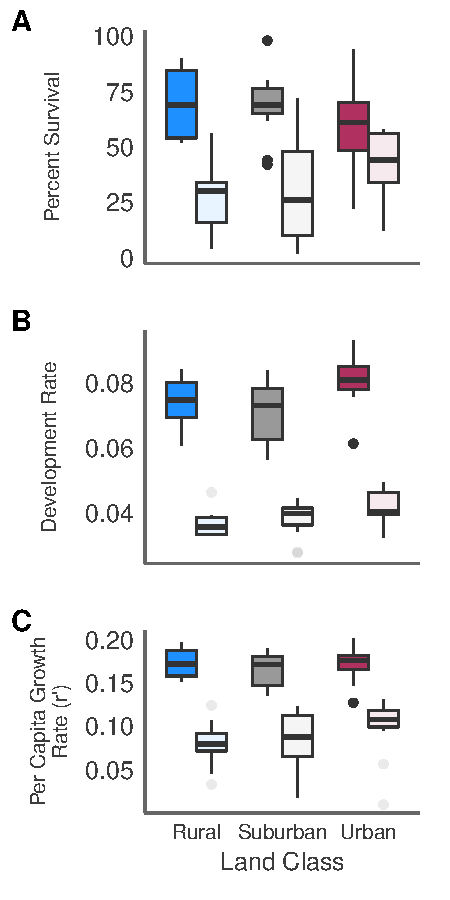
\includegraphics[height=5in, keepaspectratio]{Fig1.pdf}
\caption{Female larval a) survival rate, b) development rate and c) population growth rate across the summer (dark fill) and fall (light fill) trials and three land classes.}
\label{fig:growth}
\end{figure}

\begin{figure}
\centering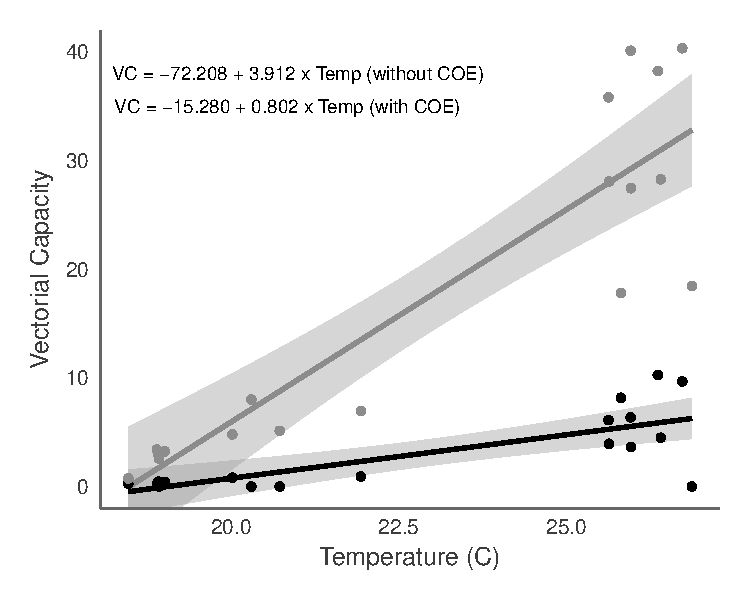
\includegraphics[height=5in, keepaspectratio]{Fig2.pdf}
\caption{Infection dynamics (infected, disseminated, and infectious mosquitoes) across land class and season. Bars represent mean and standard errors of raw data across sites (n=3 per treatment).}
\label{Fig:Infxclass}
\end{figure}

\begin{figure}
\centering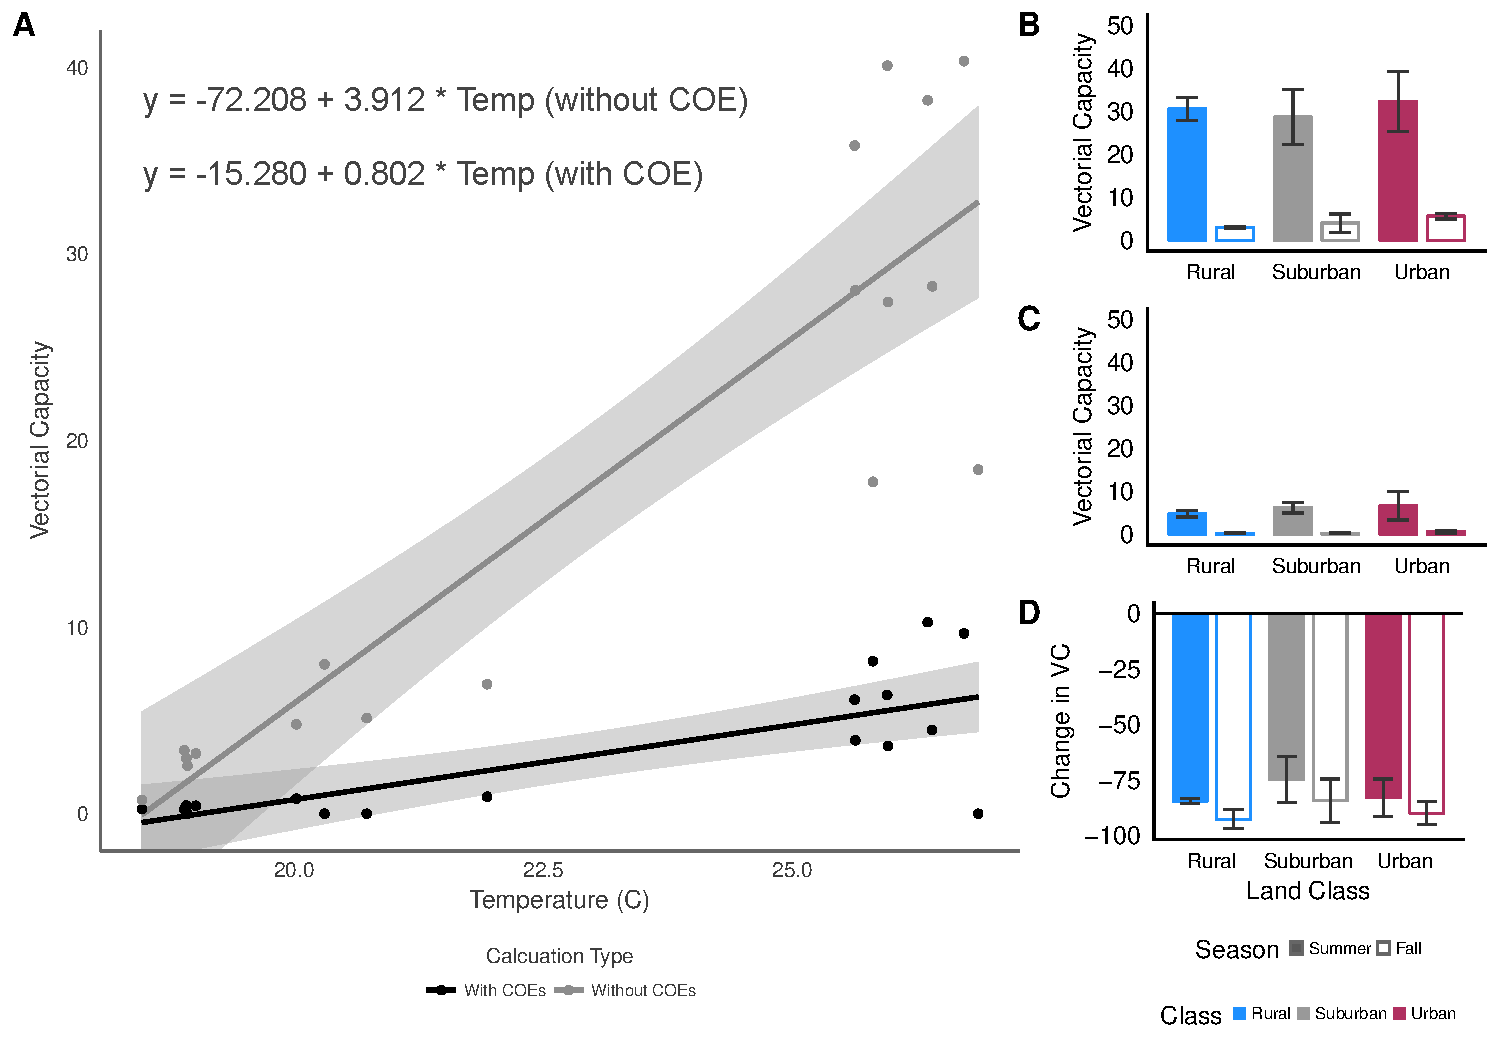
\includegraphics[width=5in]{Fig3.pdf}
\caption{The calculated vectorial capacity (with 95 \% confidence intervals) by site across individual mean temperature prior to infection assays (a). Inset charts on the right indicate calculated vectorial capacity without carry-over effects (b), with carry-over effects (c), and the percent difference due to the incorporation of carry-over effects (d). Error bars represent standard error.}
\label{Fig:VC}
\end{figure}



\end{document}
